% Options for packages loaded elsewhere
\PassOptionsToPackage{unicode}{hyperref}
\PassOptionsToPackage{hyphens}{url}
\PassOptionsToPackage{dvipsnames,svgnames,x11names}{xcolor}
%
\documentclass[
  letterpaper,
  DIV=11,
  numbers=noendperiod]{scrartcl}

\usepackage{amsmath,amssymb}
\usepackage{lmodern}
\usepackage{iftex}
\ifPDFTeX
  \usepackage[T1]{fontenc}
  \usepackage[utf8]{inputenc}
  \usepackage{textcomp} % provide euro and other symbols
\else % if luatex or xetex
  \usepackage{unicode-math}
  \defaultfontfeatures{Scale=MatchLowercase}
  \defaultfontfeatures[\rmfamily]{Ligatures=TeX,Scale=1}
\fi
% Use upquote if available, for straight quotes in verbatim environments
\IfFileExists{upquote.sty}{\usepackage{upquote}}{}
\IfFileExists{microtype.sty}{% use microtype if available
  \usepackage[]{microtype}
  \UseMicrotypeSet[protrusion]{basicmath} % disable protrusion for tt fonts
}{}
\makeatletter
\@ifundefined{KOMAClassName}{% if non-KOMA class
  \IfFileExists{parskip.sty}{%
    \usepackage{parskip}
  }{% else
    \setlength{\parindent}{0pt}
    \setlength{\parskip}{6pt plus 2pt minus 1pt}}
}{% if KOMA class
  \KOMAoptions{parskip=half}}
\makeatother
\usepackage{xcolor}
\setlength{\emergencystretch}{3em} % prevent overfull lines
\setcounter{secnumdepth}{-\maxdimen} % remove section numbering
% Make \paragraph and \subparagraph free-standing
\ifx\paragraph\undefined\else
  \let\oldparagraph\paragraph
  \renewcommand{\paragraph}[1]{\oldparagraph{#1}\mbox{}}
\fi
\ifx\subparagraph\undefined\else
  \let\oldsubparagraph\subparagraph
  \renewcommand{\subparagraph}[1]{\oldsubparagraph{#1}\mbox{}}
\fi

\usepackage{color}
\usepackage{fancyvrb}
\newcommand{\VerbBar}{|}
\newcommand{\VERB}{\Verb[commandchars=\\\{\}]}
\DefineVerbatimEnvironment{Highlighting}{Verbatim}{commandchars=\\\{\}}
% Add ',fontsize=\small' for more characters per line
\usepackage{framed}
\definecolor{shadecolor}{RGB}{241,243,245}
\newenvironment{Shaded}{\begin{snugshade}}{\end{snugshade}}
\newcommand{\AlertTok}[1]{\textcolor[rgb]{0.68,0.00,0.00}{#1}}
\newcommand{\AnnotationTok}[1]{\textcolor[rgb]{0.37,0.37,0.37}{#1}}
\newcommand{\AttributeTok}[1]{\textcolor[rgb]{0.40,0.45,0.13}{#1}}
\newcommand{\BaseNTok}[1]{\textcolor[rgb]{0.68,0.00,0.00}{#1}}
\newcommand{\BuiltInTok}[1]{\textcolor[rgb]{0.00,0.23,0.31}{#1}}
\newcommand{\CharTok}[1]{\textcolor[rgb]{0.13,0.47,0.30}{#1}}
\newcommand{\CommentTok}[1]{\textcolor[rgb]{0.37,0.37,0.37}{#1}}
\newcommand{\CommentVarTok}[1]{\textcolor[rgb]{0.37,0.37,0.37}{\textit{#1}}}
\newcommand{\ConstantTok}[1]{\textcolor[rgb]{0.56,0.35,0.01}{#1}}
\newcommand{\ControlFlowTok}[1]{\textcolor[rgb]{0.00,0.23,0.31}{#1}}
\newcommand{\DataTypeTok}[1]{\textcolor[rgb]{0.68,0.00,0.00}{#1}}
\newcommand{\DecValTok}[1]{\textcolor[rgb]{0.68,0.00,0.00}{#1}}
\newcommand{\DocumentationTok}[1]{\textcolor[rgb]{0.37,0.37,0.37}{\textit{#1}}}
\newcommand{\ErrorTok}[1]{\textcolor[rgb]{0.68,0.00,0.00}{#1}}
\newcommand{\ExtensionTok}[1]{\textcolor[rgb]{0.00,0.23,0.31}{#1}}
\newcommand{\FloatTok}[1]{\textcolor[rgb]{0.68,0.00,0.00}{#1}}
\newcommand{\FunctionTok}[1]{\textcolor[rgb]{0.28,0.35,0.67}{#1}}
\newcommand{\ImportTok}[1]{\textcolor[rgb]{0.00,0.46,0.62}{#1}}
\newcommand{\InformationTok}[1]{\textcolor[rgb]{0.37,0.37,0.37}{#1}}
\newcommand{\KeywordTok}[1]{\textcolor[rgb]{0.00,0.23,0.31}{#1}}
\newcommand{\NormalTok}[1]{\textcolor[rgb]{0.00,0.23,0.31}{#1}}
\newcommand{\OperatorTok}[1]{\textcolor[rgb]{0.37,0.37,0.37}{#1}}
\newcommand{\OtherTok}[1]{\textcolor[rgb]{0.00,0.23,0.31}{#1}}
\newcommand{\PreprocessorTok}[1]{\textcolor[rgb]{0.68,0.00,0.00}{#1}}
\newcommand{\RegionMarkerTok}[1]{\textcolor[rgb]{0.00,0.23,0.31}{#1}}
\newcommand{\SpecialCharTok}[1]{\textcolor[rgb]{0.37,0.37,0.37}{#1}}
\newcommand{\SpecialStringTok}[1]{\textcolor[rgb]{0.13,0.47,0.30}{#1}}
\newcommand{\StringTok}[1]{\textcolor[rgb]{0.13,0.47,0.30}{#1}}
\newcommand{\VariableTok}[1]{\textcolor[rgb]{0.07,0.07,0.07}{#1}}
\newcommand{\VerbatimStringTok}[1]{\textcolor[rgb]{0.13,0.47,0.30}{#1}}
\newcommand{\WarningTok}[1]{\textcolor[rgb]{0.37,0.37,0.37}{\textit{#1}}}

\providecommand{\tightlist}{%
  \setlength{\itemsep}{0pt}\setlength{\parskip}{0pt}}\usepackage{longtable,booktabs,array}
\usepackage{calc} % for calculating minipage widths
% Correct order of tables after \paragraph or \subparagraph
\usepackage{etoolbox}
\makeatletter
\patchcmd\longtable{\par}{\if@noskipsec\mbox{}\fi\par}{}{}
\makeatother
% Allow footnotes in longtable head/foot
\IfFileExists{footnotehyper.sty}{\usepackage{footnotehyper}}{\usepackage{footnote}}
\makesavenoteenv{longtable}
\usepackage{graphicx}
\makeatletter
\def\maxwidth{\ifdim\Gin@nat@width>\linewidth\linewidth\else\Gin@nat@width\fi}
\def\maxheight{\ifdim\Gin@nat@height>\textheight\textheight\else\Gin@nat@height\fi}
\makeatother
% Scale images if necessary, so that they will not overflow the page
% margins by default, and it is still possible to overwrite the defaults
% using explicit options in \includegraphics[width, height, ...]{}
\setkeys{Gin}{width=\maxwidth,height=\maxheight,keepaspectratio}
% Set default figure placement to htbp
\makeatletter
\def\fps@figure{htbp}
\makeatother
\newlength{\cslhangindent}
\setlength{\cslhangindent}{1.5em}
\newlength{\csllabelwidth}
\setlength{\csllabelwidth}{3em}
\newlength{\cslentryspacingunit} % times entry-spacing
\setlength{\cslentryspacingunit}{\parskip}
\newenvironment{CSLReferences}[2] % #1 hanging-ident, #2 entry spacing
 {% don't indent paragraphs
  \setlength{\parindent}{0pt}
  % turn on hanging indent if param 1 is 1
  \ifodd #1
  \let\oldpar\par
  \def\par{\hangindent=\cslhangindent\oldpar}
  \fi
  % set entry spacing
  \setlength{\parskip}{#2\cslentryspacingunit}
 }%
 {}
\usepackage{calc}
\newcommand{\CSLBlock}[1]{#1\hfill\break}
\newcommand{\CSLLeftMargin}[1]{\parbox[t]{\csllabelwidth}{#1}}
\newcommand{\CSLRightInline}[1]{\parbox[t]{\linewidth - \csllabelwidth}{#1}\break}
\newcommand{\CSLIndent}[1]{\hspace{\cslhangindent}#1}

\usepackage{amsmath}
\usepackage{booktabs}
\usepackage{caption}
\usepackage{longtable}
\KOMAoption{captions}{tableheading}
\makeatletter
\makeatother
\makeatletter
\makeatother
\makeatletter
\@ifpackageloaded{caption}{}{\usepackage{caption}}
\AtBeginDocument{%
\ifdefined\contentsname
  \renewcommand*\contentsname{Tabla de contenidos}
\else
  \newcommand\contentsname{Tabla de contenidos}
\fi
\ifdefined\listfigurename
  \renewcommand*\listfigurename{Listado de Figuras}
\else
  \newcommand\listfigurename{Listado de Figuras}
\fi
\ifdefined\listtablename
  \renewcommand*\listtablename{Listado de Tablas}
\else
  \newcommand\listtablename{Listado de Tablas}
\fi
\ifdefined\figurename
  \renewcommand*\figurename{Figura}
\else
  \newcommand\figurename{Figura}
\fi
\ifdefined\tablename
  \renewcommand*\tablename{Tabla}
\else
  \newcommand\tablename{Tabla}
\fi
}
\@ifpackageloaded{float}{}{\usepackage{float}}
\floatstyle{ruled}
\@ifundefined{c@chapter}{\newfloat{codelisting}{h}{lop}}{\newfloat{codelisting}{h}{lop}[chapter]}
\floatname{codelisting}{Listado}
\newcommand*\listoflistings{\listof{codelisting}{Listado de Listados}}
\makeatother
\makeatletter
\@ifpackageloaded{caption}{}{\usepackage{caption}}
\@ifpackageloaded{subcaption}{}{\usepackage{subcaption}}
\makeatother
\makeatletter
\@ifpackageloaded{tcolorbox}{}{\usepackage[many]{tcolorbox}}
\makeatother
\makeatletter
\@ifundefined{shadecolor}{\definecolor{shadecolor}{rgb}{.97, .97, .97}}
\makeatother
\makeatletter
\makeatother
\ifLuaTeX
\usepackage[bidi=basic]{babel}
\else
\usepackage[bidi=default]{babel}
\fi
\babelprovide[main,import]{spanish}
% get rid of language-specific shorthands (see #6817):
\let\LanguageShortHands\languageshorthands
\def\languageshorthands#1{}
\ifLuaTeX
  \usepackage{selnolig}  % disable illegal ligatures
\fi
\IfFileExists{bookmark.sty}{\usepackage{bookmark}}{\usepackage{hyperref}}
\IfFileExists{xurl.sty}{\usepackage{xurl}}{} % add URL line breaks if available
\urlstyle{same} % disable monospaced font for URLs
\hypersetup{
  pdflang={es},
  colorlinks=true,
  linkcolor={blue},
  filecolor={Maroon},
  citecolor={Blue},
  urlcolor={Blue},
  pdfcreator={LaTeX via pandoc}}

\author{}
\date{}

\begin{document}
\ifdefined\Shaded\renewenvironment{Shaded}{\begin{tcolorbox}[boxrule=0pt, frame hidden, borderline west={3pt}{0pt}{shadecolor}, enhanced, breakable, sharp corners, interior hidden]}{\end{tcolorbox}}\fi

\hypertarget{regresiuxf3n-ordinal}{%
\section{Regresión ordinal}\label{regresiuxf3n-ordinal}}

\hypertarget{introducciuxf3n}{%
\subsection{Introducción}\label{introducciuxf3n}}

El test de Likert es una escala ordinal. Tratar las respuestas a un test
de Likert como si fueran cuantitativas como se hizo en el análisis de la
varianza del apartado anterior no es correcto por las siguientes
razones:

\begin{itemize}
\item
  Los niveles de respuesta pueden no ser equidistantes: la distancia
  entre un par de opciones de respuesta puede no ser la misma para todos
  los pares de opciones de respuesta. Por ejemplo, la diferencia entre
  ``Muy en desacuerdo'' y ``En desacuerdo'' y la diferencia entre ``De
  acuerdo'' y ``Muy de acuerdo'' es de un nivel, pero psicológicamente
  puede ser percibida de forma diferente para cada sujeto.
\item
  La distribución de las respuestas ordinales puede ser no normal. En
  particular esto sucederá si hay frecuencias altas de respuesta en los
  extremos del cuestionario.
\item
  Las varianzas de las variables no observadas que subyacen a las
  variables ordinales observadas pueden diferir entre grupos,
  tratamientos, periodos, etc.
\end{itemize}

En Liddell y Kruschke (2018) se han analizado los problemas que puede
ocasionar tratar datos ordinales como si fueran cuantitativos
constatando que se pueden presentar las siguientes situaciones:

\begin{itemize}
\tightlist
\item
  Se pueden encontrar diferencias significativas entre grupos cuando no
  las hay: Error tipo I.
\item
  Se pueden obviar diferencias cuando en realidad sí existen: Error tipo
  II.
\item
  Incluso se pueden invertir los efectos de un tratamiento.
\item
  También puede malinterpretarse la interacción entre factores.
\end{itemize}

Todos estos problemas pueden ser tratados con la regresión ordinal.

\hypertarget{variantes-de-la-regresiuxf3n-ordinal.}{%
\subsection{Variantes de la regresión
ordinal.}\label{variantes-de-la-regresiuxf3n-ordinal.}}

Según Bürkner y Vuorre (2019) hay tres clases de regresión ordinal:

\begin{itemize}
\tightlist
\item
  Regresión ordinal acumulativa.
\item
  Regresión ordinal secuencial.
\item
  Regresión ordinal adyacente.
\end{itemize}

Nos centraremos en la primera ya que es el más habitual y adecuada para
nuestro caso.

El modelo acumulativo, CM, presupone que la variable ordinal observada,
\(Y\), proviene de la categorización de una variable latente (no
observada) continua \(\tilde{Y}\). Hay \(K\) umbrales \(\tau_k\) que
particionan \(\tilde{Y}\) en \(K + 1\) categorías ordenadas observables
(ver Figura~\ref{fig-cumulative}). Si asumimos que \(\tilde{Y}\) tiene
una cierta distribución (por ejemplo, normal) con distribución acumulada
\(F\), se puede calcular la probabilidad de que \(Y\) sea la categoría
\(k\) de esta forma:

\[Pr(Y = k) = F(\tau_k) - F(\tau_{k-1})\]

Por ejemplo en la Figura~\ref{fig-cumulative},

\[Pr(Y = 2) = F(\tau_2) - F(\tau_{1})\]

Si suponemos que, por ejemplo:

\[\tilde{Y} = \eta + \epsilon = b_1 x_1 + b_2 x_2 + \epsilon\]

Y que los errores son \(N(0,\sigma^2)\).

Entonces:

\[\mathrm{Pr}(\epsilon \leq z) = F(z)\]

Y:

\[\mathrm{Pr}(Y \leq k \mid \eta) = \mathrm{Pr}(\tilde{Y} \leq \tau_k \mid \eta) = \mathrm{Pr}(\eta + \epsilon \leq \tau k) = \mathrm{Pr}(\epsilon \leq \tau_k - \eta) = F(\tau_k - \eta)\]

Por lo que:

\[\mathrm{Pr}(Y = k) = \Phi(\tau_k - (b_1 x_1 + b_2 x_2)) - \Phi(\tau_{k - 1} - (b_1 x_1 + b_2 x_2))\]

Donde hay que estimar los umbrales y los coeficientes de regresión.

Otra popular elección es suponer que la función acumulada se comporta
como una logística. En ese caso, la interpretación de los coeficientes
varía y se asemeja a la de la regresión logística. Se parte del supuesto
de que:

\[logit (P(Y \le k)) = \tau_{k} - \eta = \tau_{k} - (b_1 x_1 + b_2 x_2)\]

Se puede demostrar que, por ejemplo:

\[\frac{\frac{\mathrm{Pr}(Y \leq k_1 \mid \eta)}{\mathrm{Pr}(Y > k_1 \mid \eta)}}{\frac{\mathrm{Pr}(Y \leq k_2 \mid \eta)}{\mathrm{Pr}(Y > k_2 \mid \eta)}} = \exp(\tau_{k_1} - \tau_{k_2})\]

\begin{figure}

{\centering 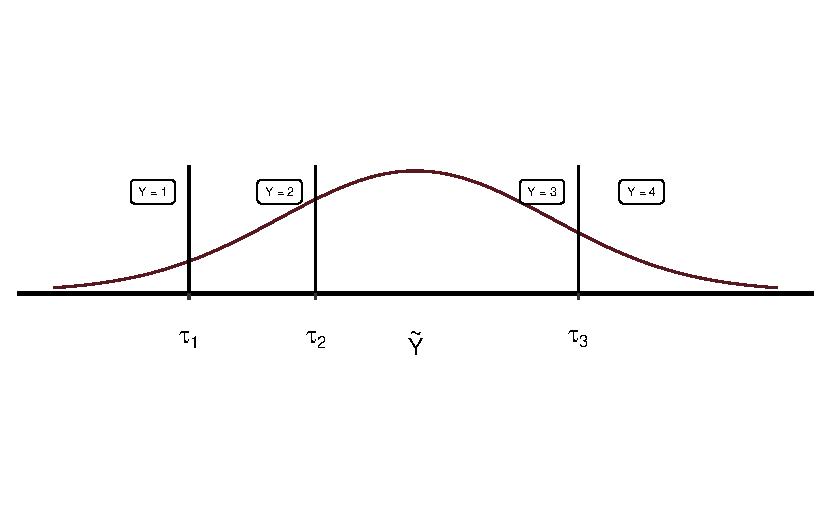
\includegraphics{ordinal_files/figure-pdf/fig-cumulative-1.pdf}

}

\caption{\label{fig-cumulative}Regresión ordinal acumulativa.}

\end{figure}

\hypertarget{preparaciuxf3n}{%
\subsection{Preparación}\label{preparaciuxf3n}}

\begin{verbatim}
Rows: 2,980
Columns: 6
$ Group    <fct> AB, AB, AB, AB, AB, AB, AB, AB, AB, AB, AB, AB, AB, AB, AB, A~
$ Period   <fct> 1, 1, 1, 1, 1, 1, 1, 1, 1, 1, 1, 1, 1, 1, 1, 1, 1, 1, 2, 2, 2~
$ Treat    <fct> A, A, A, A, A, A, A, A, A, A, A, A, A, A, A, A, A, A, B, B, B~
$ Subject  <fct> 4, 4, 4, 4, 4, 4, 4, 4, 4, 4, 4, 4, 4, 4, 4, 4, 4, 4, 4, 4, 4~
$ Question <fct> Q01, Q02, Q03, Q04, Q05, Q06, Q07, Q08, Q09, Q10, Q11, Q12, Q~
$ Response <ord> 3, 3, 3, 3, 3, 3, 3, 3, 3, 3, 3, 3, 3, 3, 3, 3, 3, 3, 3, 3, 3~
\end{verbatim}

\begin{longtable}{cccrrrrr}
\caption{Resumen de frecuencias de respuesta.}\tabularnewline

\toprule
 &  &  & \multicolumn{5}{c}{Response} \\ 
\cmidrule(lr){4-8}
Group & Period & Treat & 1 & 2 & 3 & 4 & 5 \\ 
\midrule
AB & 1 & A & 2 & 25 & 71 & 203 & 434 \\ 
AB & 2 & B & 87 & 185 & 121 & 172 & 166 \\ 
BA & 1 & B & 76 & 174 & 127 & 237 & 138 \\ 
BA & 2 & A & 2 & 30 & 64 & 345 & 321 \\ 
\bottomrule
\end{longtable}

\hypertarget{modelo-de-enlace-logit-acumulado}{%
\subsection{Modelo de enlace logit
acumulado}\label{modelo-de-enlace-logit-acumulado}}

Vamos a ajustar el modelo con la función de enlace logit:

\begin{equation}\protect\hypertarget{eq-link-logit}{}{
\text{logit} (P(y_i \leq k) = \log \frac{P(y_i \leq k)}{1 - P(y_i \leq k)}
}\label{eq-link-logit}\end{equation}

La función de enlace logit acumulada (Ecuación~\ref{eq-link-logit}) no
está definida para \(k = K\), ya que \(1 - P(Y_i \leq K) = 1 - 1 = 0\).

En nuestra escala de Likert tenemos \(K\) = 5 niveles, el modelo mixto
que vamos a plantear es el siguiente:

\[
\begin{aligned}
\text{logit}(p(y_i \leq k)) &= \tau_k - \beta_1 \text{Period}_i - \beta_2 \text{Treat}_i - \beta_3 \text{Question}_i - u( \text{Subject}_i) \\
i &= 1, \dots n \; \; \; \; \; \; k = 1, \dots, K - 1
\end{aligned}
\]

donde \(\tau_k\) es el umbral de la categoría \(k\) y son \(K-1\) = 4
interceptores. Los coeficientes de los efectos fijos, \(\beta_1\),
\(\beta_2\) y \(\beta_3\), son independientes, por lo que cada \(\beta\)
tiene el mismo efecto en los \(K-1\) logits acumulados. El efecto
aleatorio, Subject, se presupone que sigue una distribución normal:
\(u(\text{Subject}_i) \sim N(0, \sigma_u^2)\).

En esencia lo que estamos haciendo es un modelo en cadena de regresiones
logísticas donde la respuesta binaría se corresponde con ``menor o igual
que cierto nivel frente a mayor que ese nivel''.

En el caso particular de \(K\) = 5, los umbrales \(\tau_k\) se
interpretan como:

\begin{itemize}
\tightlist
\item
  \(k\) = 1: log-odds del nivel = 1 vs.~2-5
\item
  \(k\) = 2: log-odds del nivel = 1-2 vs.~3-5
\item
  \(k\) = 3: log-odds del nivel = 1-3 vs.~4-5
\item
  \(k\) = 4: log-odds del nivel = 1-4 vs.~5
\end{itemize}

\hypertarget{ajuste-del-modelo.}{%
\subsection{Ajuste del modelo.}\label{ajuste-del-modelo.}}

Vamos a usar las funciones \texttt{ordinal::clm} y
\texttt{ordinal::clmm} que respectivamente permiten ajustar modelos
únicamente con efectos fijos o modelos mixtos (efectos fijos y
aleatorios).

Comenzamos con un modelo simple que tiene un único predictor:

\[
\text{logit}(p(y_i \leq k)) = \tau_k - \beta_2 \text{Treat}_i
\]

\begin{Shaded}
\begin{Highlighting}[]
\NormalTok{clm\_likert\_treat }\OtherTok{\textless{}{-}}
    \FunctionTok{clm}\NormalTok{(}
\NormalTok{        Response }\SpecialCharTok{\textasciitilde{}}\NormalTok{ Treat,}
        \AttributeTok{data =}\NormalTok{ df, }\AttributeTok{link =} \StringTok{"logit"}
\NormalTok{    )}
\FunctionTok{summary}\NormalTok{(clm\_likert\_treat)}
\end{Highlighting}
\end{Shaded}

\begin{verbatim}
formula: Response ~ Treat
data:    df

 link  threshold nobs logLik   AIC     niter max.grad cond.H 
 logit flexible  2980 -3966.11 7942.21 5(0)  1.64e-10 3.1e+01

Coefficients:
       Estimate Std. Error z value Pr(>|z|)    
TreatB  -1.7206     0.0731  -23.54   <2e-16 ***
---
Signif. codes:  0 '***' 0.001 '**' 0.01 '*' 0.05 '.' 0.1 ' ' 1

Threshold coefficients:
    Estimate Std. Error z value
1|2 -3.97230    0.09678 -41.045
2|3 -2.45446    0.06812 -36.029
3|4 -1.66453    0.05936 -28.042
4|5 -0.10547    0.04946  -2.132
\end{verbatim}

El método \texttt{summary} muestra la información resumen. Para su
interpretación vamos a seguir Christensen (2018). La sección de
coeficientes es la más importante. Se muestra la estimación de
parámetros, el error ``stardard'' y la significación estadística de
acuerdo al test de Wald \footnote{El test de Wald es un contraste de
  hipótesis estadístico en el que se evalúa si el valor estimado es cero
  suponiendo que
  \(W = \left(\frac{\hat{\theta} - \theta_0}{se(\hat{\theta})}\right)^2 \sim \chi^{2}\)
  .}. Comprobamos que el valor es claramente significativo. Es decir,
que los estudiantes han valorado de forma diferente la calidad del
subtitulado en ambos vídeos. El estimador de maxima verosimilitud del
coeficiente \texttt{TreatB} es -1.72. La interpretación que podemos
hacer es la siguiente:

\begin{itemize}
\item
  El signo es negativo. Eso quiere decir que el subtitulado que hemos
  denominado como tratamiento B es valorado como de peor calidad por los
  estudiantes \footnote{Recuérdese que el parámetro \(\beta_2\) tiene
    signo negativo en la ecuación de regresión.}.
\item
  Los umbrales que cortan la función latente se han desplazado
  \(\beta_2\) hacia la izquierda entre el subtitulado A y B.
\item
  El \texttt{odds\ ratio} de las respuestas, \(OR(Y \geq k)\), es
  \(\exp(\widehat{\beta_2}(B - A)) = 0.18\). Siguiendo la deducción de
  (\textbf{bruin?}) podemos, por ejemplo, hacer la siguiente
  interpretación del significado de este coeficiente referido a dos
  niveles consecutivos de respuesta:
\end{itemize}

\[
\begin{aligned}
logit (P(Y \le 1)) & = & -3.97 - -1.72 x_2 \\
logit (P(Y \le 2)) & = & -2.45 - -1.72 x_2
\end{aligned}
\]

Por lo tanto los \texttt{odds} serían:

\[
\begin{aligned}
\frac{P(Y \le 1 | x_2 = B)}{P(Y \gt 1 | x_2 = B)} & = & exp(-3.97)/exp(-1.72) \\
\frac{P(Y \le 1 | x_2 = A)}{P(Y \gt 1 | x_2 = A)} & = & exp(-3.97) \\
\frac{P(Y \le 2 | x_2 = B)}{P(Y \gt 2 | x_2 = B)} & = & exp(-2.45)/exp(-1.72) \\
\frac{P(Y \le 2 | x_2 = A)}{P(Y \gt 2 | x_2 = A)} & = & exp(-2.45)
\end{aligned}
\]

El número de condición Hessiano es inferior a \(10^4\) lo que es
indicativo de que no hay problemas de optimización \footnote{El número
  de condición de Hessiano es una medida de la curvatura de una función
  en un punto. Si el número de condición de Hessiano es grande, la
  función es muy sensible a pequeñas perturbaciones y puede ser difícil
  de optimizar.}.

Añadimos un segundo predictor para constatar si existe efecto periodo.

\[
\text{logit}(p(y_i \leq k)) = \tau_k - \beta_1 \text{Period}_i - \beta_2 \text{Treat}_i
\]

\begin{Shaded}
\begin{Highlighting}[]
\NormalTok{clm\_likert\_period\_treat }\OtherTok{\textless{}{-}}
    \FunctionTok{clm}\NormalTok{(}
\NormalTok{        Response }\SpecialCharTok{\textasciitilde{}}\NormalTok{ Period }\SpecialCharTok{+}\NormalTok{ Treat,}
        \AttributeTok{data =}\NormalTok{ df, }\AttributeTok{link =} \StringTok{"logit"}
\NormalTok{    )}
\FunctionTok{summary}\NormalTok{(clm\_likert\_period\_treat)}
\end{Highlighting}
\end{Shaded}

\begin{verbatim}
formula: Response ~ Period + Treat
data:    df

 link  threshold nobs logLik   AIC     niter max.grad cond.H 
 logit flexible  2980 -3957.88 7927.76 5(0)  1.93e-10 4.1e+01

Coefficients:
        Estimate Std. Error z value Pr(>|z|)    
Period2 -0.27560    0.06805   -4.05 5.12e-05 ***
TreatB  -1.74090    0.07339  -23.72  < 2e-16 ***
---
Signif. codes:  0 '***' 0.001 '**' 0.01 '*' 0.05 '.' 0.1 ' ' 1

Threshold coefficients:
    Estimate Std. Error z value
1|2 -4.13085    0.10507 -39.314
2|3 -2.60905    0.07872 -33.143
3|4 -1.81652    0.07073 -25.681
4|5 -0.25187    0.06153  -4.093
\end{verbatim}

Vemos que ambos coeficientes son significativos y con signo negativo. Un
signo negativo en el efecto periodo está asociado a que la valoración
del subtitulado empeora en el segundo periodo independientemente de si
se trata del subtitulado correcto o incorrecto.

Podemos comparar ambos modelos con la prueba de razón de verosimilitud y
comprobamos que el modelo con efecto periodo reduce la función de
verosimilitud y, por lo tanto, debe ser aceptado:

\begin{Shaded}
\begin{Highlighting}[]
\FunctionTok{anova}\NormalTok{(clm\_likert\_treat, clm\_likert\_period\_treat)}
\end{Highlighting}
\end{Shaded}

\begin{verbatim}
Likelihood ratio tests of cumulative link models:
 
                        formula:                  link: threshold:
clm_likert_treat        Response ~ Treat          logit flexible  
clm_likert_period_treat Response ~ Period + Treat logit flexible  

                        no.par    AIC  logLik LR.stat df Pr(>Chisq)    
clm_likert_treat             5 7942.2 -3966.1                          
clm_likert_period_treat      6 7927.8 -3957.9  16.448  1      5e-05 ***
---
Signif. codes:  0 '***' 0.001 '**' 0.01 '*' 0.05 '.' 0.1 ' ' 1
\end{verbatim}

Con la función \texttt{drop1} se puede realizar este mismo test, razón
de verosimilitudes, para cada la variable explicativa del modelo
controlando las restantes.

\begin{Shaded}
\begin{Highlighting}[]
\FunctionTok{drop1}\NormalTok{(clm\_likert\_period\_treat, }\AttributeTok{test =} \StringTok{"Chi"}\NormalTok{)}
\end{Highlighting}
\end{Shaded}

\begin{verbatim}
Single term deletions

Model:
Response ~ Period + Treat
       Df    AIC    LRT Pr(>Chi)    
<none>    7927.8                    
Period  1 7942.2  16.45    5e-05 ***
Treat   1 8537.8 612.03   <2e-16 ***
---
Signif. codes:  0 '***' 0.001 '**' 0.01 '*' 0.05 '.' 0.1 ' ' 1
\end{verbatim}

Y con la función \texttt{add1}, que hace el test de cada variable
explicativa ignorando las restantes:

\begin{Shaded}
\begin{Highlighting}[]
\CommentTok{\# Fit the null model first}
\NormalTok{clm\_likert\_null }\OtherTok{\textless{}{-}} \FunctionTok{clm}\NormalTok{(Response }\SpecialCharTok{\textasciitilde{}} \DecValTok{1}\NormalTok{, }\AttributeTok{data =}\NormalTok{ df, }\AttributeTok{link =} \StringTok{"logit"}\NormalTok{)}
\FunctionTok{add1}\NormalTok{(clm\_likert\_null, }\AttributeTok{scope =} \SpecialCharTok{\textasciitilde{}}\NormalTok{ Period }\SpecialCharTok{+}\NormalTok{ Treat, }\AttributeTok{test =} \StringTok{"Chi"}\NormalTok{)}
\end{Highlighting}
\end{Shaded}

\begin{verbatim}
Single term additions

Model:
Response ~ 1
       Df    AIC    LRT Pr(>Chi)    
<none>    8541.7                    
Period  1 8537.8   5.91  0.01504 *  
Treat   1 7942.2 601.49  < 2e-16 ***
---
Signif. codes:  0 '***' 0.001 '**' 0.01 '*' 0.05 '.' 0.1 ' ' 1
\end{verbatim}

En la Figura~\ref{fig-clm_likert_period_treat-confint} se muestran los
intervalos de confianza de los parámetros del modelo.

\begin{figure}

{\centering 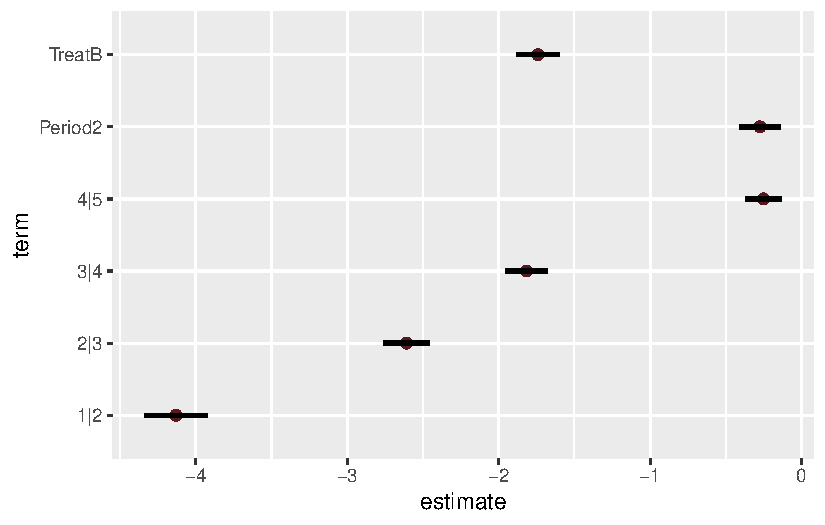
\includegraphics{ordinal_files/figure-pdf/fig-clm_likert_period_treat-confint-1.pdf}

}

\caption{\label{fig-clm_likert_period_treat-confint}Intervalos de
confianza}

\end{figure}

El \(OR\) de los parámetros es:

\begin{longtable}{lrrr}
\toprule
term & estimate & conf.low & conf.high \\ 
\midrule
1|2 & $0.02$ & $0.01$ & $0.02$ \\ 
2|3 & $0.07$ & $0.06$ & $0.09$ \\ 
3|4 & $0.16$ & $0.14$ & $0.19$ \\ 
4|5 & $0.78$ & $0.69$ & $0.88$ \\ 
Period2 & $0.76$ & $0.66$ & $0.87$ \\ 
TreatB & $0.18$ & $0.15$ & $0.20$ \\ 
\bottomrule
\end{longtable}

Modelo con interacción entre periodo y subtítulos:

\[
\text{logit}(p(y_i \leq k)) = \tau_k - \beta_1 \text{Period}_i - \beta_2 \text{Treat}_i - \beta_3 \text{Period}_i\text{Treat}_i
\]

\begin{Shaded}
\begin{Highlighting}[]
\NormalTok{clm\_likert\_period\_treat\_inter }\OtherTok{\textless{}{-}}
    \FunctionTok{clm}\NormalTok{(}
\NormalTok{        Response }\SpecialCharTok{\textasciitilde{}}\NormalTok{ Period }\SpecialCharTok{*}\NormalTok{ Treat,}
        \AttributeTok{data =}\NormalTok{ df, }\AttributeTok{link =} \StringTok{"logit"}
\NormalTok{    )}
\FunctionTok{summary}\NormalTok{(clm\_likert\_period\_treat\_inter)}
\end{Highlighting}
\end{Shaded}

\begin{verbatim}
formula: Response ~ Period * Treat
data:    df

 link  threshold nobs logLik   AIC     niter max.grad cond.H 
 logit flexible  2980 -3953.01 7920.03 5(0)  2.12e-10 8.1e+01

Coefficients:
               Estimate Std. Error z value Pr(>|z|)    
Period2        -0.49179    0.09744  -5.047 4.49e-07 ***
TreatB         -1.96046    0.10229 -19.166  < 2e-16 ***
Period2:TreatB  0.42510    0.13638   3.117  0.00183 ** 
---
Signif. codes:  0 '***' 0.001 '**' 0.01 '*' 0.05 '.' 0.1 ' ' 1

Threshold coefficients:
    Estimate Std. Error z value
1|2 -4.24649    0.11182 -37.977
2|3 -2.72823    0.08821 -30.928
3|4 -1.93833    0.08167 -23.732
4|5 -0.36991    0.07308  -5.062
\end{verbatim}

\begin{Shaded}
\begin{Highlighting}[]
\FunctionTok{anova}\NormalTok{(clm\_likert\_period\_treat, clm\_likert\_period\_treat\_inter)}
\end{Highlighting}
\end{Shaded}

\begin{verbatim}
Likelihood ratio tests of cumulative link models:
 
                              formula:                  link: threshold:
clm_likert_period_treat       Response ~ Period + Treat logit flexible  
clm_likert_period_treat_inter Response ~ Period * Treat logit flexible  

                              no.par    AIC  logLik LR.stat df Pr(>Chisq)   
clm_likert_period_treat            6 7927.8 -3957.9                         
clm_likert_period_treat_inter      7 7920.0 -3953.0   9.738  1   0.001805 **
---
Signif. codes:  0 '***' 0.001 '**' 0.01 '*' 0.05 '.' 0.1 ' ' 1
\end{verbatim}

Vemos que hay evidencia de que existe una interacción entre periodo y
subtítulos. Cuando esto sucede se tiende a dar mayor importancia a esta
interacción que a los efectos principales de cada factor.

\hypertarget{modelo-con-efectos-mixtos}{%
\subsubsection{Modelo con efectos
mixtos}\label{modelo-con-efectos-mixtos}}

\begin{Shaded}
\begin{Highlighting}[]
\NormalTok{clmm\_likert\_period\_treat\_inter\_subject }\OtherTok{\textless{}{-}}
    \FunctionTok{clmm}\NormalTok{(}
\NormalTok{        Response }\SpecialCharTok{\textasciitilde{}}\NormalTok{ Period }\SpecialCharTok{*}\NormalTok{ Treat }\SpecialCharTok{+}\NormalTok{ (}\DecValTok{1} \SpecialCharTok{|}\NormalTok{ Subject),}
        \AttributeTok{data =}\NormalTok{ df, }\AttributeTok{link =} \StringTok{"logit"}
\NormalTok{    )}
\FunctionTok{summary}\NormalTok{(clmm\_likert\_period\_treat\_inter\_subject)}
\end{Highlighting}
\end{Shaded}

\begin{verbatim}
Cumulative Link Mixed Model fitted with the Laplace approximation

formula: Response ~ Period * Treat + (1 | Subject)
data:    df

 link  threshold nobs logLik   AIC     niter     max.grad cond.H 
 logit flexible  2980 -3655.71 7327.41 635(2507) 3.16e-04 5.8e+02

Random effects:
 Groups  Name        Variance Std.Dev.
 Subject (Intercept) 1.278    1.131   
Number of groups:  Subject 87 

Coefficients:
               Estimate Std. Error z value Pr(>|z|)    
Period2         -0.5985     0.2652  -2.257    0.024 *  
TreatB          -2.3926     0.2672  -8.954   <2e-16 ***
Period2:TreatB   0.5705     0.5070   1.125    0.260    
---
Signif. codes:  0 '***' 0.001 '**' 0.01 '*' 0.05 '.' 0.1 ' ' 1

Threshold coefficients:
    Estimate Std. Error z value
1|2  -5.0575     0.2154 -23.481
2|3  -3.3828     0.2014 -16.794
3|4  -2.4541     0.1969 -12.461
4|5  -0.5248     0.1909  -2.749
\end{verbatim}

Vemos que ahora la interacción periodo y tratamiento en no
significativa.

\begin{Shaded}
\begin{Highlighting}[]
\NormalTok{clmm\_likert\_period\_treat\_subject }\OtherTok{\textless{}{-}}
    \FunctionTok{clmm}\NormalTok{(}
\NormalTok{        Response }\SpecialCharTok{\textasciitilde{}}\NormalTok{ Period }\SpecialCharTok{+}\NormalTok{ Treat }\SpecialCharTok{+}\NormalTok{ (}\DecValTok{1} \SpecialCharTok{|}\NormalTok{ Subject),}
        \AttributeTok{data =}\NormalTok{ df, }\AttributeTok{link =} \StringTok{"logit"}
\NormalTok{    )}
\FunctionTok{summary}\NormalTok{(clmm\_likert\_period\_treat\_subject)}
\end{Highlighting}
\end{Shaded}

\begin{verbatim}
Cumulative Link Mixed Model fitted with the Laplace approximation

formula: Response ~ Period + Treat + (1 | Subject)
data:    df

 link  threshold nobs logLik   AIC     niter     max.grad cond.H 
 logit flexible  2980 -3656.34 7326.67 516(2067) 3.66e-04 1.1e+02

Random effects:
 Groups  Name        Variance Std.Dev.
 Subject (Intercept) 1.296    1.139   
Number of groups:  Subject 87 

Coefficients:
        Estimate Std. Error z value Pr(>|z|)    
Period2 -0.31159    0.07204  -4.325 1.52e-05 ***
TreatB  -2.10685    0.07997 -26.344  < 2e-16 ***
---
Signif. codes:  0 '***' 0.001 '**' 0.01 '*' 0.05 '.' 0.1 ' ' 1

Threshold coefficients:
    Estimate Std. Error z value
1|2  -4.9122     0.1713 -28.669
2|3  -3.2370     0.1533 -21.110
3|4  -2.3079     0.1473 -15.670
4|5  -0.3786     0.1399  -2.706
\end{verbatim}

\begin{Shaded}
\begin{Highlighting}[]
\FunctionTok{anova}\NormalTok{(clmm\_likert\_period\_treat\_subject, clmm\_likert\_period\_treat\_inter\_subject)}
\end{Highlighting}
\end{Shaded}

\begin{verbatim}
Likelihood ratio tests of cumulative link models:
 
                                       formula:                                 
clmm_likert_period_treat_subject       Response ~ Period + Treat + (1 | Subject)
clmm_likert_period_treat_inter_subject Response ~ Period * Treat + (1 | Subject)
                                       link: threshold:
clmm_likert_period_treat_subject       logit flexible  
clmm_likert_period_treat_inter_subject logit flexible  

                                       no.par    AIC  logLik LR.stat df
clmm_likert_period_treat_subject            7 7326.7 -3656.3           
clmm_likert_period_treat_inter_subject      8 7327.4 -3655.7    1.26  1
                                       Pr(>Chisq)
clmm_likert_period_treat_subject                 
clmm_likert_period_treat_inter_subject     0.2617
\end{verbatim}

\begin{Shaded}
\begin{Highlighting}[]
\NormalTok{clmm\_likert\_period\_treat\_subject\_question }\OtherTok{\textless{}{-}}
    \FunctionTok{clmm}\NormalTok{(}
\NormalTok{        Response }\SpecialCharTok{\textasciitilde{}}\NormalTok{ Period }\SpecialCharTok{+}\NormalTok{ Treat }\SpecialCharTok{+}\NormalTok{ (}\DecValTok{1} \SpecialCharTok{|}\NormalTok{ Subject) }\SpecialCharTok{+}\NormalTok{ (}\DecValTok{1} \SpecialCharTok{|}\NormalTok{ Question),}
        \AttributeTok{data =}\NormalTok{ df, }\AttributeTok{link =} \StringTok{"logit"}
\NormalTok{    )}

\FunctionTok{summary}\NormalTok{(clmm\_likert\_period\_treat\_subject\_question)}
\end{Highlighting}
\end{Shaded}

\begin{verbatim}
Cumulative Link Mixed Model fitted with the Laplace approximation

formula: Response ~ Period + Treat + (1 | Subject) + (1 | Question)
data:    df

 link  threshold nobs logLik   AIC     niter     max.grad cond.H 
 logit flexible  2980 -3560.09 7136.19 835(3344) 1.58e-03 1.8e+02

Random effects:
 Groups   Name        Variance Std.Dev.
 Subject  (Intercept) 1.4546   1.2061  
 Question (Intercept) 0.3395   0.5827  
Number of groups:  Subject 87,  Question 18 

Coefficients:
        Estimate Std. Error z value Pr(>|z|)    
Period2 -0.32029    0.07286  -4.396  1.1e-05 ***
TreatB  -2.23815    0.08226 -27.208  < 2e-16 ***
---
Signif. codes:  0 '***' 0.001 '**' 0.01 '*' 0.05 '.' 0.1 ' ' 1

Threshold coefficients:
    Estimate Std. Error z value
1|2  -5.1745     0.2269 -22.801
2|3  -3.4120     0.2121 -16.087
3|4  -2.4161     0.2070 -11.672
4|5  -0.3715     0.2012  -1.847
\end{verbatim}

\begin{Shaded}
\begin{Highlighting}[]
\FunctionTok{anova}\NormalTok{(clmm\_likert\_period\_treat\_subject, clmm\_likert\_period\_treat\_subject\_question)}
\end{Highlighting}
\end{Shaded}

\begin{verbatim}
Likelihood ratio tests of cumulative link models:
 
                                          formula:                                                  
clmm_likert_period_treat_subject          Response ~ Period + Treat + (1 | Subject)                 
clmm_likert_period_treat_subject_question Response ~ Period + Treat + (1 | Subject) + (1 | Question)
                                          link: threshold:
clmm_likert_period_treat_subject          logit flexible  
clmm_likert_period_treat_subject_question logit flexible  

                                          no.par    AIC  logLik LR.stat df
clmm_likert_period_treat_subject               7 7326.7 -3656.3           
clmm_likert_period_treat_subject_question      8 7136.2 -3560.1  192.48  1
                                          Pr(>Chisq)    
clmm_likert_period_treat_subject                        
clmm_likert_period_treat_subject_question  < 2.2e-16 ***
---
Signif. codes:  0 '***' 0.001 '**' 0.01 '*' 0.05 '.' 0.1 ' ' 1
\end{verbatim}

\hypertarget{predicciones}{%
\subsection{Predicciones}\label{predicciones}}

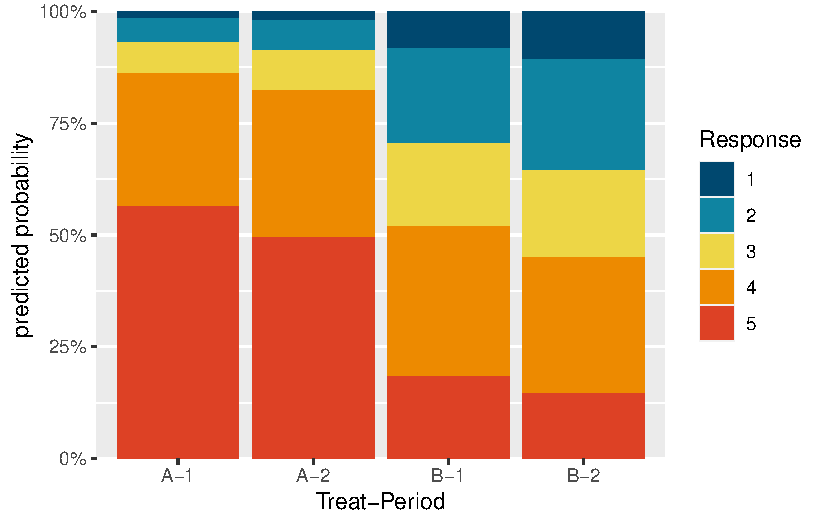
\includegraphics{ordinal_files/figure-pdf/unnamed-chunk-24-1.pdf}

\begin{verbatim}
$`emmeans of Period`
 Period emmean    SE  df asymp.LCL asymp.UCL
 1        1.72 0.198 Inf      1.34      2.11
 2        1.40 0.197 Inf      1.02      1.79

Results are averaged over the levels of: Treat 
Confidence level used: 0.95 

$`pairwise differences of Period`
 1                 estimate     SE  df z.ratio p.value
 Period1 - Period2     0.32 0.0729 Inf   4.396  <.0001

Results are averaged over the levels of: Treat 

$`emmeans of Treat`
 Treat emmean    SE  df asymp.LCL asymp.UCL
 A      2.683 0.202 Inf    2.2883     3.078
 B      0.445 0.195 Inf    0.0625     0.828

Results are averaged over the levels of: Period 
Confidence level used: 0.95 

$`pairwise differences of Treat`
 1     estimate     SE  df z.ratio p.value
 A - B     2.24 0.0823 Inf  27.208  <.0001

Results are averaged over the levels of: Period 
\end{verbatim}

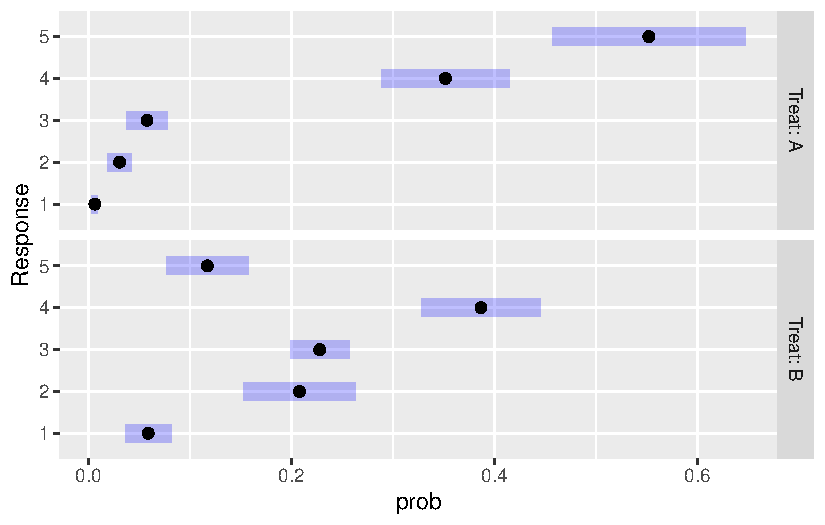
\includegraphics{ordinal_files/figure-pdf/unnamed-chunk-26-1.pdf}

\hypertarget{refs}{}
\begin{CSLReferences}{1}{0}
\leavevmode\vadjust pre{\hypertarget{ref-burkner}{}}%
Bürkner, Paul-Christian, y Matti Vuorre. 2019. {«Ordinal Regression
Models in Psychology: A Tutorial»}. \emph{Advances in Methods and
Practices in Psychological Science} 2 (1): 77-101.
\url{https://doi.org/10.1177/2515245918823199}.

\leavevmode\vadjust pre{\hypertarget{ref-christensen2018CumulativeLM}{}}%
Christensen, Rune Haubo Bojesen. 2018. {«Cumulative Link Models for
Ordinal Regression with the R Package ordinal»}. En.

\leavevmode\vadjust pre{\hypertarget{ref-kruschke2018328}{}}%
Liddell, Torrin M., y John K. Kruschke. 2018. {«Analyzing ordinal data
with metric models: What could possibly go wrong?»} \emph{Journal of
Experimental Social Psychology} 79: 328-48.
https://doi.org/\url{https://doi.org/10.1016/j.jesp.2018.08.009}.

\end{CSLReferences}



\end{document}
